% =============================================================================
% P3A -- Privacy 2: poster (EN), style2 version
% Style of the P2A poster (_grupo/P2A/mainV3.tex): a0poster A1 portrait, UnB mark,
% green small-caps title, two columns with numbered blue headings, no boxes.
% Figures expected in out/: Fig1_EN.pdf, Fig2_EN.pdf, Fig4_EN.pdf (built from figuras/).
% UnB mark: figuras/marca_unb.png. Content equals P3A_Privacidade2_Poster_EN.tex.
% =============================================================================
\documentclass[a1,portrait]{a0poster}
\usepackage[brazil,english]{babel}
\usepackage[utf8]{inputenc}
\usepackage[absolute]{textpos}
\usepackage{graphicx}
\usepackage{color}
\usepackage{xcolor}
\usepackage{amsmath,amssymb}
\usepackage{booktabs}

\definecolor{DarkBlue}{rgb}{0.1,0.1,0.5}
\definecolor{Red}{rgb}{0.9,0.0,0.1}
\definecolor{DarkGreen}{rgb}{0.10,0.50,0.10}

\let\Textsize\normalsize
\def\LHead#1{\noindent{\LARGE\color{DarkBlue} #1}\smallskip}
\def\Subhead#1{\noindent{\large\color{DarkBlue} #1}}
\newcommand{\quiteHuge}{\fontsize{55}{70}\selectfont}
\def\Title#1{\begin{center}\noindent{\quiteHuge\color{DarkGreen}#1}\end{center}}

\TPGrid[40mm,40mm]{23}{12}

\parindent=0pt
\parskip=0.5\baselineskip

\begin{document}
\large

\begin{textblock}{23}(0,0)
\centering

\includegraphics[width=18cm]{figuras/marca_unb.png}
\end{textblock}

\begin{textblock}{23}(0,0.5)
\Title{\textsc{Privacy in PMBOK 8: a proposed performance domain for the Who concentration}}
\end{textblock}

\begin{textblock}{23}(0,1.1)
\begin{center}
  \parbox{0.8\textwidth}{
    \small
    \begin{center}
    \textbf{Authors:} Filipe Alves de Sousa, Emanuel Brandão de Galvão Correia, Ruben Isaac Dias da Silva and Carlos Eduardo da Silva Papa\\
    \textbf{Course:} IT Project Management (GPTI) -- PPCA/CIC/UnB\\
    \textbf{Professors:} Dr. João Mello da Silva and Dr. Edison Ishikawa\\
    \textbf{Deliverable:} P3A | \textbf{Code:} 3p2 / 3R31
    \end{center}
  }
\end{center}
\end{textblock}

% ------------------------------- LEFT COLUMN ----------------------------------
\begin{textblock}{11}(0,2.0)

\LHead{1. Problem and proposal}

PMBOK 8 [14] mentions data protection and privacy, but its seven domains and 40 processes do not organize personal-data processing as a distinct management object. We propose \textbf{Privacy} in the \textbf{Who} concentration, alongside Stakeholders and Risk.

\textbf{Guiding question:} how might project data practices affect people, and what evidence supports the project's choices?

\vspace{0.3cm}
\LHead{2. Where Privacy fits}

\begin{figure}[h!]
\centering
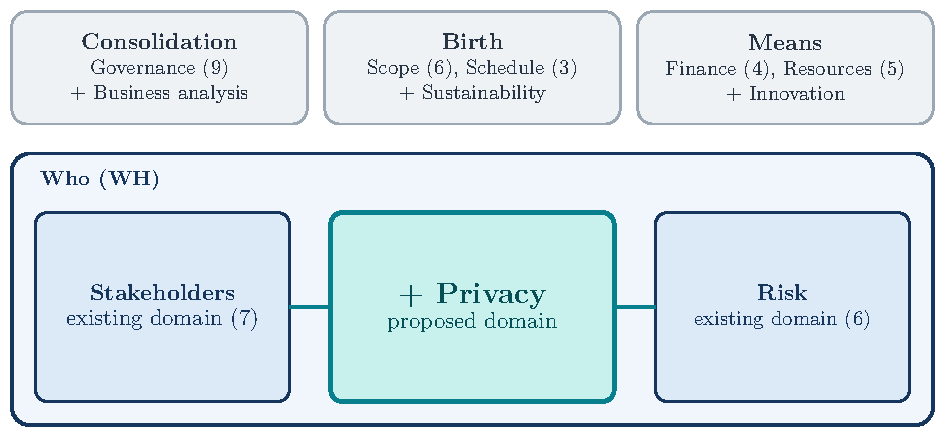
\includegraphics[width=\linewidth]{out/Fig1_EN.pdf}
\caption{Position of the proposed domain among the concentrations.}
\end{figure}

The four concentrations are the organization adopted in this work. \textbf{Privacy} is the group's contribution to the \textbf{Who} concentration.

\vspace{0.3cm}
\LHead{3. Alignment with the 6 principles}

\textbf{1AHV} End-to-end view of data flows\\
\textbf{2FOV} Benefits weighed against potential harms\\
\textbf{3QPD} Privacy as verifiable quality\\
\textbf{4BAL} Accountable decisions and owners\\
\textbf{5SPA} Lasting effects on people\\
\textbf{6BEC} Channels for challenge and learning

\vspace{0.3cm}
\LHead{4. Eight proposed processes: decision and evidence}

{\small
\begin{itemize}
    \item \textbf{P1 Identify subjects and data} $\rightarrow$ initial inventory.
    \item \textbf{P2 Define purposes and roles} $\rightarrow$ privacy plan.
    \item \textbf{P3 Assess impacts on people} $\rightarrow$ assessment; DPIA if warranted.
    \item \textbf{P4 Choose proportionate responses} $\rightarrow$ control plan.
    \item \textbf{P5 Inform and route requests} $\rightarrow$ response records.
    \item \textbf{P6 Apply controls and handle incidents} $\rightarrow$ implementation evidence.
    \item \textbf{P7 Review effectiveness and new purposes} $\rightarrow$ plan update.
    \item \textbf{P8 Decide retention, transfer, or deletion} $\rightarrow$ disposition record.
\end{itemize}
}

\end{textblock}

% ------------------------------- RIGHT COLUMN ---------------------------------
\begin{textblock}{11}(12,2.0)

\LHead{5. Privacy across the project}

\begin{figure}[h!]
\centering
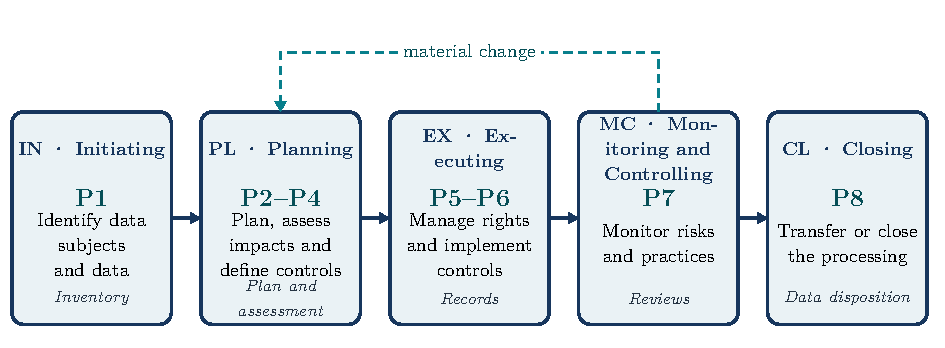
\includegraphics[width=\linewidth]{out/Fig2_EN.pdf}
\caption{Privacy across the project.}
\end{figure}

P1--P8 are \textbf{group-proposed processes} across the five focus areas. The return arrow indicates reassessment; data processing may continue after project closure.

\vspace{0.3cm}
\LHead{6. Digital twins and data exposure}

\begin{figure}[h!]
\centering
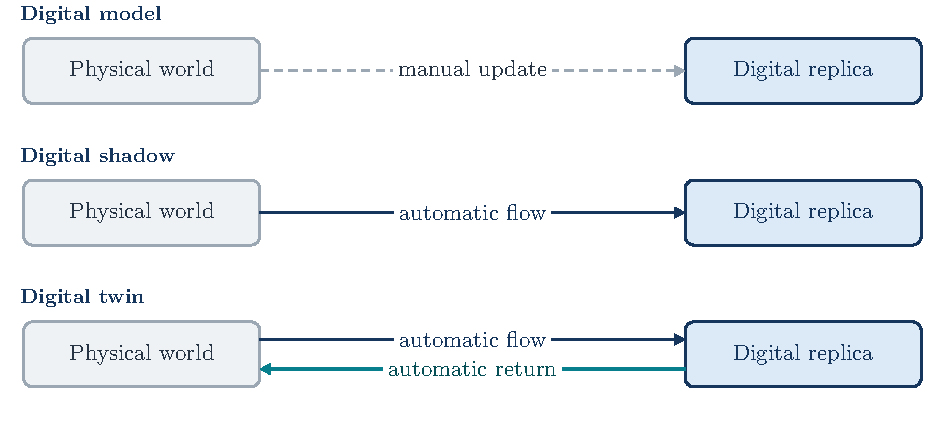
\includegraphics[width=\linewidth]{out/Fig4_EN.pdf}
\caption{Digital twins and data exposure.}
\end{figure}

The classification follows Kritzinger et al. [12]. Automatic, frequent flows call for attention to data subjects, purposes, sharing, risks, and data disposition [17].

\vspace{0.3cm}
\LHead{7. Key references}

{\normalsize
[12] KRITZINGER, W. et al. Digital twin in manufacturing: a categorical literature review and classification. \textbf{IFAC-PapersOnLine}, vol. 51, no. 11, 2018.

[14] PMI. \textbf{The Standard for Project Management and A Guide to the PMBOK (PMBOK Guide)}. 8th ed., 2025.

[17] WANG, Y. et al. A survey on digital twins: architecture, enabling technologies, security and privacy, and future prospects. \textbf{IEEE Internet of Things Journal}, vol. 10, no. 17, 2023.

\textit{Numbering of the full report.}
% \textit{P1--P8 are an academic proposal and are not official PMBOK 8 processes.}  % NOTA-COMENTADA
}

\end{textblock}

% AVISO-IA:INICIO
\begin{textblock}{23}(0,11.4)
{\small\noindent \textbf{AI use:} generative AI (ChatGPT Astral 6 Sol and Sonnet 5.5, high mode) supported text editing, formatting, figure creation, and table drafting. The group is responsible for the content (COPE, 2023: \texttt{publicationethics.org/guidance/cope-position/authorship-and-ai-tools}).\par}
\end{textblock}
% AVISO-IA:FIM

\end{document}
